\chapter{Úvod}

V době vysokorychlostního a stabilního internetu je využívání vzdálených uložišť běžnou záležitostí. Pro většinu uživatelů je to nástroj
pro jednoduchou synchronizaci dat napříč několika zařízeními od mobilního telefonu po stolní počítač. Pokud vezmeme v úvahu pouze velká datová centra,
jedná se pravděpodobně o nejlevnější a nejspolehlivější způsob uchování dat, protože tyto centra mají velkou kapacitu úložného prostoru a také zálohy na
softwarové i hardwarové úrovni. Pod pojmem vzdálené uložiště si nemusíme představit jen velká datová centra se stovkami serverů, může se jednat o relativně malé uložiště
ve firmě nebo dokonce o osobní/domácí řešení. Pro využívaní osobních/firemních uložišť se lidé uchylují v případech, je-li třeba uložit osobní nebo
určitým způsobem citlivá data, která by nemohla být poskytnuta třetí straně. Nabízená řešení také nemusí poskytovat potřebnou funkcionalitu nebo jejich finanční model
nesplňuje zákazníkova kritéria.

V průběhu let byly vyvinuty protokoly řešící sdílení souborů jako FTP, NFS a mnohé další. Sdílení souborů je komplexní záležitostí a obsahuje
velké množství parametrů. Každý protokol se zaměřuje jen na určité parametry jako zabezpečení a spolehlivost přenosu, oprávnění pro jednotlivé
uživatele a soubory, synchronizace modifikovaných souborů apod nebo pojme daný parametr odlišným způsobem. V dnešní době je většina komerčně využívaných
aplikací vystavěna na proprietárních protokolech nebo na protokolech umožňující obecnější použití. Jedním z nejpoužívanějších aplikačních protokolů
bude Hypertext Transfer Protokol neboli HTTP.

Cílem této práce je prozkoumat aktuální nabídku a možnosti na poli vzdálených uložišť a navrhnout aplikaci pro řízený přístup ke vzdáleným dokumentům pro
platformu \mbox{GNU/Linux}. Aplikace bude zaměřena na řízený životní cyklus souborů s vynucenými oprávněními pro jednotlivé soubory daná vzdáleným uložištěm.
Komunikace skrze HTTP protokol byla definovaná externím zadavatelem. Zdrojové kódy jsou dostupné na veřejném Github repozitáři.
\footnote{\url{https://github.com/PlayerBerny12/VUT-IBT-Code}}

% ---------------------------------------------------------------------------------------------------------------------------------------
\chapter{Motivace a existující řešení}

Popularita a využití vzdálených uložišť roste, protože lidé využívají více zařízení a potřebují mezi nimi jednoduchou synchronizaci nebo na jednom souboru
potřebuje spolupracovat více lidí. Dalším podnětem využívání vzdálených uložišť je většího množství dat a potřeba tyto data efektivně sdílet a bezpečně uložit.
Postupně se digitalizují další systémy například ve státní správě nebo dalších podnikatelských sektorech. 

Na trhu je velké množství služeb zaměřujících se na různé klientské potřeby. Diverzita nabídky je až překvapivě velká. Většina se zaměřuje na ukládání a sdílení
dat ve svém ekosystému, které jsou určené pro široké použití. Pokud jsou požadavky specifické, tak možnost vlastní konfigurace není možná. Pro částečnou úpravu 
nebo automatizaci procesů lze využít poskytované API, ve většině případu se jedná o variantu REST API. Poslední možností je vystavění obdobné služby z několika
existujících aplikací nebo vytvoření nové.\\

\noindent V kontextu této práce jsou požadavky následující: 

\begin{itemize}
    \item Dodržování oprávnění i na klientském systému
    \begin{itemize}
        \item read-only
        \item write-only
        \item read/write
    \end{itemize}
    \item Životní cyklus souboru (stažení)
    \begin{itemize}
        \item stažení
        \item případná modifikace
        \item smazání souboru po vypršení platnosti
    \end{itemize}
    \item Autentifikace
    \begin{itemize}
        \item uživatelské jméno a klientský certifikát
        \item uživatelské jméno a heslo
    \end{itemize}
\end{itemize}

\section{Současná řešení}

Pro bližší analýzu byl vybrán vzorek služeb a programů obsahující velké ekosystémy služeb po open source aplikace. Zkoumáno bylo několik parametrů,
jako poskytovaná funkcionalita pro jednotlivce a firmy, cena, integrace s ostatními systémy a aplikacemi apod. Obecně nelze jednoznačně určit nejlepší uložiště, 
ale je možné poukázat na rozdílné vlastnosti a vyzdvihnout kladné. Koncový uživatel se následně může rozhodnout dle svých potřeb.

\section{Google Drive}

Pro synchronizaci obsahu z Google Drive na osobní počítač se využívá aplikace pojmenovaná Google File Stream. Je možné ji provozovat pouze na systémech
Windows a Mac OS.\cite{GoogleFileStream} Pro Linuxové distribuce lze využít například neoficiální open source aplikaci 
Google Drive OCamlFUSE\footnote{\url{https://github.com/astrada/google-drive-ocamlfuse}} využívající technologii
FUSE, která bude popsána v následující kapitole \ref{sec:fuse}. Google Disk poskytuje plně funkční webové rozhraní,
ve kterém je možné dokumenty přímo upravovat bez nutnosti stahování. Problém nenastal ani v případě konkurenčních Microsoft Office dokumentů. 

Google Workspace (dříve Google Suite) je možné pořídit v několika balíčcích. Například balíček Bussiness Standard nabízí 2 TB uložiště za 10,40 EUR měsíčně.
Balíček obsahuje další služby jako firemní email a schůzky až o 150 účastnících na Google Meet.\cite{GoogleWorkspace}

Každý uživatel má vlastní disk s omezenou kapacitou podle balíčku. Na disku lze vytvářet standartní složkovou hierarchii a je možné sdílet jednotlivé soubory nebo
obsah složek s ostatními Google uživateli. Verze Enterprise umožňuje vytváření dalších disků, na které je možné přiřadit seznam uživatelů. Každý uživatel
má nastavenou jednu z 6 rolí, které vymezují jeho možnosti. K dispozici je API, která pokrývá veškeré možnosti webového rozhraní jako vytvoření souboru,
sdílení atd.\cite{GoogleAPIReference}

\section{Dropbox}

Dropbox má oficiální balíčky své aplikace pro Ubuntu a Fedoru, případně je možné si aplikaci zkompilovat ze zdrojových souborů. Podpora Windows a Mac OS je samozřejmostí.
Z práce „Personal Cloud Storage Benchmarks and Comparison“ lze vyčíst, že Dropbox se zaměřuje na efektivitu přenosu a minimální zatížení sítě.
Využívá menší množství TCP spojení oproti jeho konkurentům a také stejně jako Google Drive komprimuje data před odesláním.\cite{CloudStorageComparison}
Toto řešení nemusí dosahovat nejvyšší výkonosti, ale nezatěžuje tolik infrastrukturu. 

Webové rozhraní je více orientováno na správu souborů a jejich historii. Nabízí jednoduché obnovení smazaných souborů nebo návrat k předchozí verzi.
Nenabízí tolik možností jako Google Drive, ale upravovat dokumenty ve webovém prohlížeči lze také. Na výběr je mezi Microsoft Office Online nebo Google Worksapce.
Sdílení souborů a složek je možné i s uživateli, kteří nemají Dropbox účet.

Balíček Plus za 9,99 EUR měsíčně dává uživateli přístup ke 2 TB uložišti. Firemní balíčky obsahují rozšíření pro lepší správu uživatelů, vytváření skupin
a admin panel/konzole. Dropbox má také API nabízející dostatečnou funkcionalitu pro případnou integraci s jinými systémy apod.\cite{Dropbox}

\section{pCloud}

Poskytovatel pCloud podporuje nejpoužívanější platformy, a to včetně mobilních. Za 9,99 EUR měsíčně dostane uživatel 2 TB uložiště. Jako jediný z poskytovatelů
v analýze nabízí balíček s jednorázovou platbou za cenu 350 EUR. Jedná se o identický balíček, pouze forma platby se liší. Všechna data jsou přenášena přes
šifrovaný kanál a všechny kopie souborů na pěti různých serverech jsou šifrovaná 256bitovým AES klíčem.\cite{pCloud}

Webové rozhraní je jednoduché, avšak oproti konkurentům má méně funkcí. Lze zobrazit náhled dokumentů, ale upravovat je nelze. Každý soubor má tzv. revize 
a je možné obnovit obsah souboru na vybranou revizi. Revize jsou uchovány po dobu jednoho roku. Soubory je možné sdílet i s uživateli, kteří nemají účet u pCloudu. 

Pro firemní zákazníky je nabízený rozšířený management uživatelů a monitoring s logy aktivity jednotlivých uživatelů.

\section{Syncthing}

Open source aplikace Syncthing synchronizuje soubory peer-to-peer. Nejedná se o čistou peer-to-peer architekturu, protože jeden z uzlů může být
nastaven jako server a veškeré data budou synchronizována vůči tomuto uzlu. Syncthing je možné provozovat na většině dnešních systémů jako Windows, Linux, BSD a
Mac OS.\cite{Syncthing}

Aplikace poskytuje webové rozhraní, které je určené pouze pro nastavení parametrů jako discovery protokol pro objevování ostatních uzlů, jaké složky mají být synchronizovány
nebo kolik verzí jednotlivých souborů má být uchováváno a mnoho dalšího. Velká přizpůsobivost umožňuje upravit fungování aplikace vlastním potřebám, na druhou
stranu bude náročné udržovat systém s větším množstvím uživatelů vystavěný na této aplikaci. Jedná se tedy spíše o domácí řešení.

\section{Shrnutí}

Trendy na poli vzdálených uložišť určují velké firmy jako Google nebo Micorsoft. Důkazem tohoto jevu je například integrace aplikací obou těchto firem do webového
rozhraní Dropboxu. Aplikace One Drive od Microsoftu nebyla blíže analyzovaná, protože se jedná o službu pouze pro platformu Windows. 

Všechny služby mají webové rozhraní, ke kterému je aplikace synchronizující obsah uložiště občas braná jako doplňek. Sdílení nebo obnova předchozí verze souboru
je vždy možná ve webové aplikaci, ale ne vdžy jsou tyto akce dostupné i na desktopové verzi.

Aplikace na jejíž základě je vytvořená tato práce nebude synchronizovat celé uložiště, ale bude pracovat jen s jednotlivými soubory. Uživateli na vyžádání stáhne 
právě jeden soubor, se kterým bude chtít uživatel v danou dobu pracovat (zobrazit nebo upravit obsah). Synchromizace celého uložiště nebo obasahu jedné složky nebude možná.
Jedná se spíše o náhradu možnosti zobrazovat a upravovat soubor přímo ve webovém prohlížeči jako to umožňuje například Google Drive.

% ---------------------------------------------------------------------------------------------------------------------------------------
\chapter{Návrh řešení a použité technologie}

Prvním krokem navrhovací fáze bylo seznámení se zadáním a požadavky. Externí zadavatel dodal podrobnou dokumentaci REST API pro validované datové uložiště, která
byla stěžejním dokumentem při návrhu. Jednalo se formální textový popis, který nebyl v žádném standardizovaném formát. API obsahuje funkce pro ověření spojení,
autentifikaci a práci se soubory. VDU nebylo při vzniku této práce k dispozic a proto byl pro potřeby vývoje vytvořen mock server na základě přepisu poskytnuté
dokumentace do standardizovaného formátu OpenAPI.

Pro vynucení práv jednotlivých souborů je standartní souborový systém nevyhovující, protože po stažení souboru do počítače uživatele ztrácí VDU kontrolu nad tímto
souborem. Po konzultaci s vedoucím práce, dokterem Markem Rychlým, byla zvolena technologie FUSE neboli Filesystem in userspace. FUSE umožňuje vytvořit virtuální
souborový systém a implementovat jednotlivé operace jako čtení, zápis atd. Tím je možné dosáhnout dostatečnou kontrolu nad oprávněními a obecně životním cyklem souboru
v uživatelově počítači. Znalý uživatel by byl schopen tento systém obejít a přistoupit k souborům z hostovaného souborového systému. K takové operaci jsou potřeba 
oprávnění superuživatele \texttt{root}.

\section{Případy užití}

Ze zadání bylo možné přímo vytvořit diagram případu užití, pouze jedna věc nebyla specifikovaná. Webová aplikace musí předat desktopové přístupový token, 
pomocí kterého lze udělat potřebné API volání na VDU. V úvahu přišlo stažení „fake“ souboru obsahující pouze přístupový token. Druhou možností bylo
přesměrování na speciální URL z VDU. Prohlížeč by na základě přesměrování rozpoznal, že má otevřít určenou aplikaci a předat ji token jako jeden z
parametrů volání. Varainta se speciální URL působí na uživatele mnohem ucelenějším dojmem a nevytváří na souorovém systém dále nepotřebné soubory.

Diagram případu užití zachycuje celý systém jako celek a zobrazuje jednotlivé funkce a jejich návaznosti, které je třeba dále analyzovat a specifikovat v dalších
fázích návrhu. V diagramu \ref{fig:use_case} vystupují tři aktéři a to uživatel, FUSE agent/démon a VDU. Implementace VDU není obsahem této práce, proto je oddělena červenou
přerušovanou čarou. V diagramu není zanesená například autentifikace, na které závisí veškerá komunikace s VDU. Pro přehlednost byla tato část vypuštěna.

\begin{figure*}[h]
    \centering    
    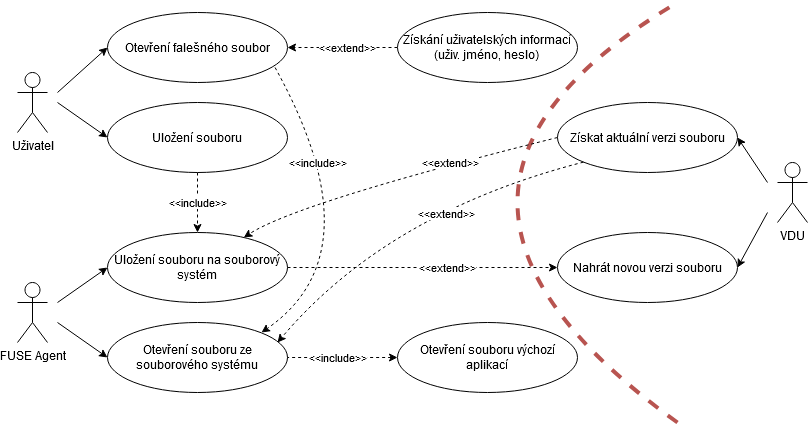
\includegraphics[width=1\linewidth]{other-fig/use_case_diagram.png}
    \caption{Diagram případu užití}
    \label{fig:use_case}
\end{figure*}


Všechny akce jsou spuštěny uživatelem a většina z nich vyvolá reakci FUSE démona. Jedná se například o uložení, otevření nebo přejmenování souboru ve virtuálním souborovém
systému. Speciální případ nastává při otevření URL s vlastním protokolem, který má zavolat aplikaci, jež je k danému protokolu v systému přiřazena. Příkladem takového
protokolu může být \texttt{mailto}, využívaný často u webových stránek. Přesměrování na adresu s tímto protokolem otevře správce elektronické pošty. 

K námi definovanému protokolu pojmenovaném \texttt{vdu} je třeba mít v systému přiřazenou aplikaci, která s přístupovým tokenem uloženým v URL 
(\texttt{vdu://<přístupový token>}) stáhne žádaný soubor z VDU na virtuální souborový systém. Na základě této znalosti byly uskutečněny rozhodnutí při návrhu architektury.
 
\section{Definice REST API}

API obsahuje sedm metod pro ověření dostupnosti, autentifikaci a práci se se soubory. Každá funkce má sadu možných návratových hodnot indikující jestli dané volání
bylo úspešné nebo proč dané volání selhalo.

\begin{itemize}
    \item /ping - 
    \begin{itemize}
        \item GET /ping - pro ověření dostupnosti VDU        
    \end{itemize}
    \item /auth
    \begin{itemize}
        \item GET /auth/key - obnova autentifikačního tokenu
        \item POST /auth/key - získání autentifikačního tokenu
        \item DELETE /auth/key - zneplatnění autentifikačního tokenu
    \end{itemize}
    \item /file
    \begin{itemize}
        \item GET /file/<file-access-token> - stažení obsahu souboru
        \item POST /file/<file-access-token> - nahrání obsahu souboru
        \item DELETE /file/<file-access-token> - zneplatnění přístupového tokenu
    \end{itemize}
\end{itemize}

Standardizace definice REST API byla vytvořena v OpenAPI standardu, pro který je dostupných mnoho nástrojů. Jedním z nich je open source nástroj Swagger, pomocí kterého
můžete generovat html dokumentaci. Vygenerované rozhraní umožňuje i jednoduchou formu testování API. Pomocí standartdizované definice bylo také možné rychle vytvořit 
mock server ve webové aplikaci Postman.

\section{Architektura}

Zvažovány byly dvě implementační varianty, jedna verze pracoval pouze s FUSE démonem a druhá rozdělila funkčnost do samostatné aplikace a FUSE démona. První variantu by
bylo možné zpracovat dvěma obdobnými způsoby vedoucí ke stejnému řešení. FUSE démon je napsaný v jazyce C, takže jedno z nabízejících se řešení by byla implementace
celé aplikace jednom jazyce. Druhým řešením by bylo vytvoření C++ knihovny, která by měla interface pro jazyk C. Tudíž by vytvořená knihovna mohla být konzumována FUSE démonem.
Nejedná se však o nijak kriticky náročnou aplikaci na výkon, takže by varianta s C++ knihovnou byla upřednostňovaná, protože standartní knihovna jazyka C++ a jeho konstrukce 
umožňují jednodušší vývoj.

Rozdělení na dvě samostatné aplikace z nichž jedna je FUSE démon by mohlo přinést problémy v udržitelnosti takového systému. Pokud by jedna z aplikací nefungovala, celý systém
by nemohl pracovat korektně. Hlavní aplikace by obsluhovala komunikaci s VDU a byla by vždy spuštěna voláním z FUSE démona nebo nepřímo uživatelem. Se znalostí 
získanou při návrhu diagramu případů užití víme, že je třeba mít registrovanou aplikaci obsluhující otevření speciální URL. I kdybychom vzali místo URL soubor se speciální
koncovkou (např. *.vdu) obsahující přístupový token je stále třeba mít přiřazenou aplikaci pro obsluhu tentokrát otvírání souboru. Démon běžící na pozadí po celou dobu běhu
systému nemůže být přiřazen jako aplikace obsluhující takové události. Na základě těchto okolností byla vybrána varianta se dvěma oddělenýmí aplikacemi.

\begin{figure*}[h]
    \centering
    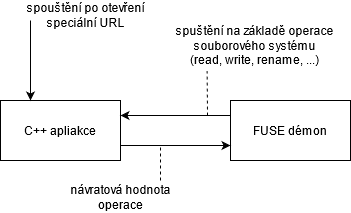
\includegraphics[width=0.47\linewidth]{other-fig/architecture.png}
    \caption{Architektura}
\end{figure*}

Pokud FUSE démon má vykonat akci, pro kterou nemá dostatečné informace, spustí jako další subproces druhou hlavní aplikaci a počká na návratovou hodnotu, na základě
které se rozhodne, jakým způsobem onu akci dokončí. Může se jednat o situace jako: je soubor určený jen pro četní nebo i zápis, je daný soubor stále validní
validní (nevypršel datum expirace) apod.

V této variantě je FUSE démon velmi minimalistický a zybtek funkcionality je implementován v druhé aplikaci, která běží jen pokud je k tomu vyzvaná, narozdíl od neustále
běžícího démona. Démon tedy po celou dobu běhu zabírá méně místa, protože nemusí mít načtené v paměti všechny potřebné knihovny. Tyto knihovny mohou být v paměti i tak
namapované, protože je mohou využívat jiné aplikace. Démon musí být spuštěný s oprávněními superuživatele \texttt{root} a menší množství kódu běžícího s vysokými
oprávněními implikuje menší náchylnost na bezpečnostní chyby. Hlavní aplikace může běžet jen s právy přihlášeného uživatele.

\subsection{Diagram tříd}

Aby implementace probíhala s možná nejmenším množstvím komplikací a nebylo třeba již uvažovat nad dalšími rozhodnutími, byl vytvořen diagram tříd \ref{fig:class_diagram_design},
který se pokouší podrobně vizualizovat třídy s atributy a metodami, jež je třebe implementovat. Jedná se pouze o návrh, který se v průběhu vývoje bude měnit, ale pokud je návrh
kvalitní a programátoři se jej sanží dodržet, neměl by být výsledek zásadně rozdílný.

\begin{figure*}[h]
    \centering
    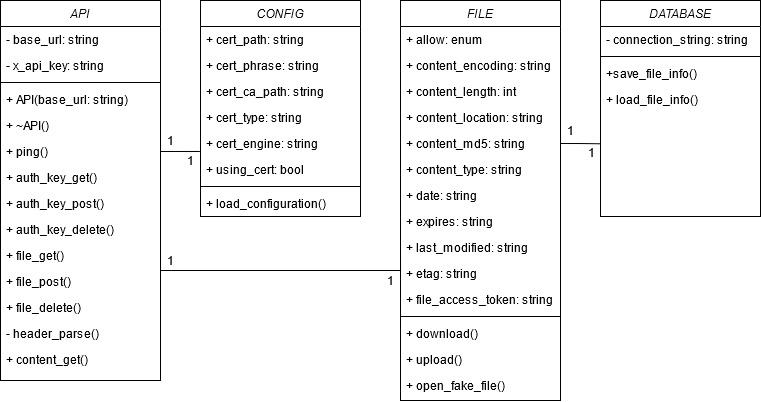
\includegraphics[width=1\linewidth]{other-fig/class_diagram_design.png}
    \caption{Diagram tříd - návrh}
    \label{fig:class_diagram_design}
\end{figure*}

Na obrázku \ref{fig:class_diagram_implementation} je možné vidět diagram tříd naimplementovaného programu. Na první pohled vypadá velmi rozdílně, po bližším prozkoumáním
lze vidět jednu novou třídu oproti návrhu. Jedná se o třídu zobrazující notifikace pro uživatele, která nemá vliv na hlavní funkcionalitu. Dále přibylo několik podpůrných
funkcí a také přibili některé atributy, případně se přejmenovali. Při implementaci nenastaly žádné zásadní potíže způsobené chybným nebo nepřesným návrhem, tudíž lze
návrh označit za úspěšný.

\newpage

\begin{figure*}[h]
    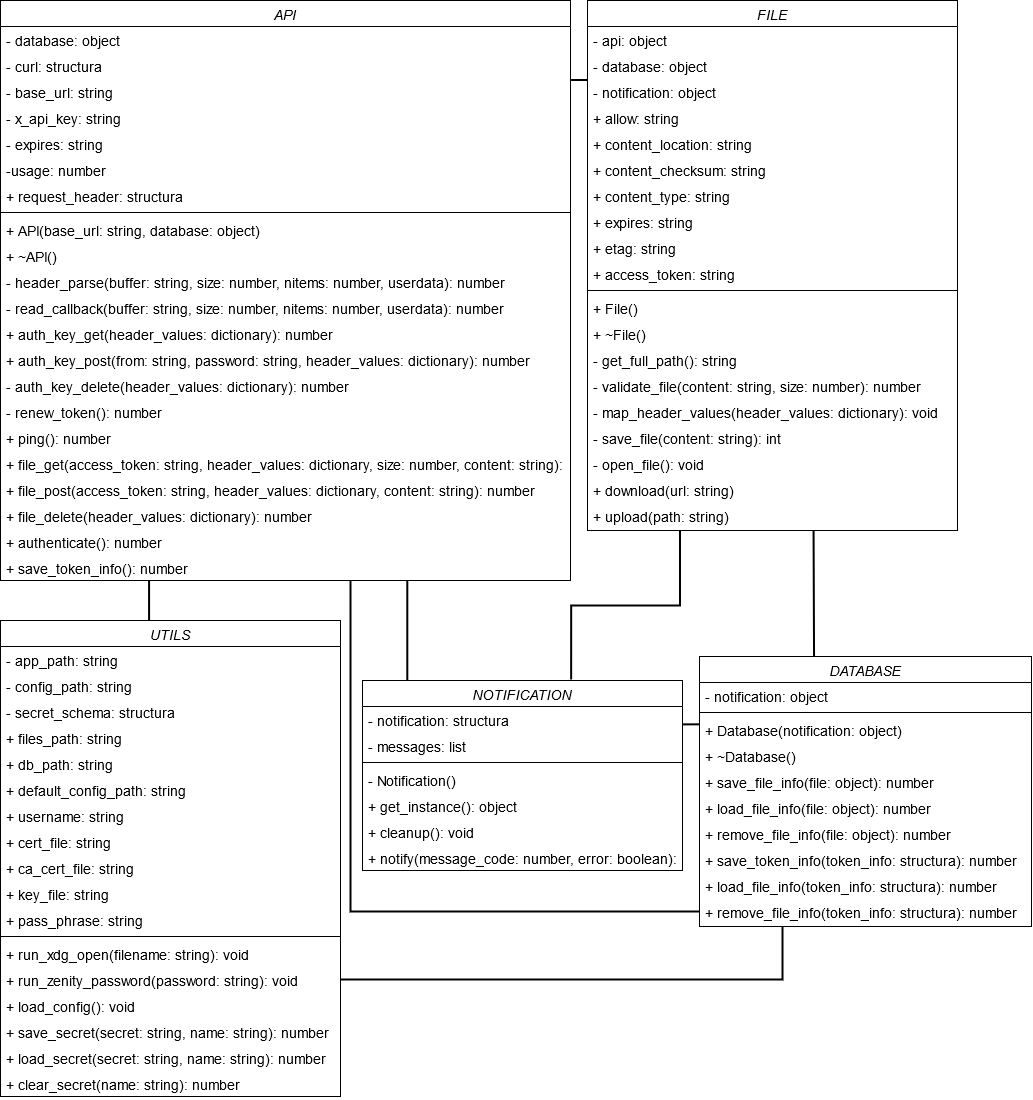
\includegraphics[width=1\linewidth]{other-fig/class_diagram_after_implementation.png}
    \caption{Diagram tříd - implementace}
    \label{fig:class_diagram_implementation}
\end{figure*}

\section{Technologie}

V této sekci budou popsány jednotlivé technologie, které ovlivnili tuto práci. Pro samotný návrh stačí elementární znalosti daných technologií, ale pro
implementaci a jejich správné využití je třeba jejich bližší pochopení.

\subsection{GNU/Linux}

GNU je rekurzivní zkratka pro „GNU's Not Unix!“. Jedná se o projekt, který měl za cíl vystavět nový operační systém kompatipilní s Unixem. Všechen kód vytvořený pod
tímto projektem je tzv. free software (svobodný software). Jedná se o filosofii vývoje software jejíž parafrázovaná definice je následující. Svobodný (free) software se
vztahuje ke svobodě, ne k ceně. Slovo svobodný (free) by mělo být bráno ve významu svobodný projev (free speech) nikoliv pivo zdarma (free beer) \cite{FreeSoftware}.

V projektu GNU postupně vznikali jednotlivé softwareové balíky, které měli ve výsledku poskládat nový operační systém. Pod projektem GNU vnikli aplikace jako překladač GCC,
textový fomátovač TeX, terminálový shell Bash a mnohé další. Na počátku 90. let byl systém téměř hotový, jediné co scházelo bylo jádro. Ve stejném období dokončoval
Linus Torvalds své jádro operačního systému nazývané Linux.\cite{GNULinux}\cite{GNULinux2} 

Tak vznikla myšlenka tyto dva projekty spojit a vnikl GNU/Linux. Balíčky projektu GNU umožnovali práci se systémem postaveným nad Linuxovým jádre. Všechny dnešní distribuce
jako jsou Debian, Fedora a další jsou distribuce systému GNU/Linux. Linux je název pouze jádra pro operační systém, který zevšeobecněl a je tímto názvem chybně označováno
celý systém. Projekt GNU dodnes vyvýjí své jádro pojmenované GNU Hurd, se kterým by vznikl operační systém GNU, což byl počáteční cíl projektu.\cite{GNULinux2}

\subsection{C++/C}

Jazyk C patří do skupiny dlouho používaných programovacích jazyků. Se svoji bohatou historií sahající až do 70. let 20. století velmi ovlivnil další nástupnické procedurální
jazyky jako C++, C\#, Java atd. V roce 1989 byl jazyk standardizován jako ANSI C a následně přišli ISO standardy označované jako C99, C11, C17. Patří mezi vysokoúrovňové
programovací jazyky, přestože se jedná o relativně jednoduchý programoací jazyk obsahující malé množství konstrukcí.\cite{CReference}

Vývoj C++ je oproti C dynamičtější, což můžeme vidět na jednotlivých ISO standardech C++98, C++03, C++11, C++14, C++17 a C++20. Jazyk C++ se v poslední dekádě velmi
proměnil a období od standardu C++11 je označováno za doubu „moderního C++“. V posledním standardu přibyla podpora konceptů nebo rozsahů.\cite{CPPReference}

Při využití překladačů GCC nebo G++ lze využít tzv. GNU rozšiřující standardy. Poté je možné využít některé konstrukce, které nejsou specifikované v oficiálním ISO standardu.
V případě jazyka C se jedná o standary pojmenované GNU99, GNU11 a GNU17, v případě C++ se jedná o GNU++11 a jemu podobné.

\subsection{HTTP}

Hypertext Transfer Protokol je protokol aplikační vrsty TCP/IP stacku. Byl vytvořen pro přenášení hypertextových souborů v 90. letech 20. století a dnes se jedná o
nejrozšířenější aplikační protokol. Poslední stabilní verze protokolu je označená jako HTTP/2 vydaná v roce 2015. Aktuálně je ve fázi specifikace nástupce pojmenovaný HTTP/3.

HTTP v čisté formě se dnes moc nepoužívá, ale využívá se ve spojení s TLS. Při komunikaci se nejprve vytvoří TCP spojení a poté šifrovaný kanál, skrze který je HTTP
bezpečně přenášeno. Toto řešení není nejefektivnější, protože vznikalo postupně a spojovali se technologie, které nebyly od počátku navržené pro tento účel. Ve většině případů
uživatel nepozná co se děje pod povrchem, ale takovéto spojení například trpí dlouho časovou prodlevou, než se ustálí pro přenášení dat. Tento problém má vyřršit právě nová
verze HTTP.\cite{HTTP3}

\begin{figure*}[h]
    \centering
    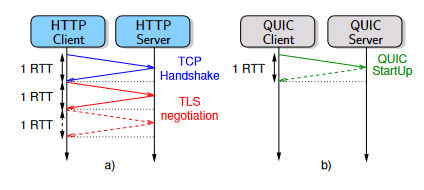
\includegraphics[width=0.8\linewidth]{other-fig/http_comparison.png}
    \caption{Porovnání HTTP verze 2 (a) a 3 (b). Převzato z „HTTP over UDP: An Experimental Investigation of QUIC“\cite{HTTP3}}
    \label{fig:http_comparison}
\end{figure*}

Nová verze využívá nový protokol QUIC, který využívá protokol UDP namísto TCP jako tomu bylo u předchozích verzích HTTP. Na obrázku \ref{fig:http_comparison} je možné vidět,
že navázání komunikace je ze tří výměn informací zredukováno jen na jednu. Formát hlavičky by měl zůstat nezměněný a tudíž je zpětně kompatipilní.

Pro tento projekt je důležitá práce s datumy a jejich formáty v HTTP hlavičce. RFC7231 specifikuje tři formáty datumů, z nichž dva jsou označené jako zastaralé,
ale jsou stále validní.\cite{RFC7231}

\begin{itemize}
    \item Upřednostňovaný formát
    \begin{itemize}
        \item Sun, 06 Nov 1994 08:49:37 GMT (IMF-fixdate formát)
    \end{itemize}
    \item Zastaralé formáty
    \begin{itemize}
        \item Sunday, 06-Nov-94 08:49:37 GMT (RFC 850 formát)
        \item Sun Nov  6 08:49:37 1994 (ANSI C asctime() formát)
    \end{itemize}
\end{itemize}

\subsection{OpenAPI}

Jedná se o standard pro definování metod REST API, ketrý má v čase psaní této práce poslední verzi 3.0.3. Zápis je možný ve dvou jazycích a to JSON a YAML. Oba 
je možné strojově zpracovat a přitom jsou pro člověka stále čitelné. 

Specifikace je velmi obsáhlá a umožňuje popsat API velmi detailně a přitom efektivně. Například je možné vytvářet šablony datových strukturu, které jsou používány jako
vstupní nebo naopak návratová hodnoty jednotlivých funkcí. V definici je pak možné na tuto šablonu odkázat. Struktura souboru je hierarchcká a skládá se z jednotlivých objektů.
Každý objekt má povinné a volitelné atributy. Definovat tedy lze hlavičky požadavku, URL query parametry, návratové kódy a k nim přiřazená návratové hlavičky a odpovědi.
Toto byl jen stručný minimální výpis, co je možné pomocí tohoto standardu definovat.\cite{OpenAPI}

\subsection{Mock server}

- testovací vzor mock serveru

\cite{MockServer}

\subsection{Souborový systém v uživatelském prostoru (FUSE)}
\label{sec:fuse}

- co je to fuse
- jak funguje (démon, blokové zařízení, ...)
- operace, které je možné implementovat
    - minimálně potřebné operace pro funkční fuse

\cite{FuseOrNotToFuse}
\cite{HardeningFUSE}

\subsection{DBus}

- co to je 
- jaké systémové služby je možné přes to ovládat

\subsection{Keyring}

- co to je
- jak to funguje
- implementace (gnom-kering, kde-wallet, linux-keyring)
    - odlišnosti implemnetací

\cite{Keyring}

% ---------------------------------------------------------------------------------------------------------------------------------------
\chapter{Popis implementace a nasazení aplikace}

- Seznam použitých knihoven

\section{Definice API}
\section{Mock server}
\section{Vyžívané cesty/soubory v Linuxové adresářové struktuře}
\subsection{Konfigurační soubor}
\subsection{SQLite databáze}
\section{Autentifikace}
\section{Práce se soubory}
\subsection{Otevření souboru v příslušné aplikaci}

\cite{xdg}

\section{Nasazení aplikace}
\subsection{DPKG} %APT
\subsection{RPM} %DNF/YUM
\subsection{Sestavení ze zdrojových souborů}

% ---------------------------------------------------------------------------------------------------------------------------------------
\chapter{Testovací sada}

- Testy pro funkce třídy API

\section{Google Test}

% ---------------------------------------------------------------------------------------------------------------------------------------
\chapter{Závěr}



